%----------------------------------------------------------------------------------------
%	DOCUMENT CONFIGURATIONS
%----------------------------------------------------------------------------------------
\documentclass[11pt]{article}

\usepackage{float}
\usepackage{caption}
\usepackage{subcaption}
\usepackage{cleveref}

\RequirePackage{amsmath}
\RequirePackage{amssymb}
\RequirePackage{amsthm}
\usepackage{amsfonts}
\usepackage{mathtools}

\usepackage{epsfig}
\usepackage{amscd}
\usepackage{graphicx}% Include figure files
\usepackage{dcolumn}% Align table columns on decimal point
\usepackage{bm}% bold math
\usepackage{enumerate}
\usepackage{tikz}


\usepackage[top=1.5in,bottom=1.5in,right=1.5in, left=1.5in]{geometry}

\captionsetup[subfigure]{subrefformat=simple,labelformat=simple}
\renewcommand\thesubfigure{(\alph{subfigure})}

%----------------------------------------------------------------------------------------
%	TITLE SECTION
%----------------------------------------------------------------------------------------



%----------------------------------------------------------------------------------------
%	ARTICLE SECTION
%----------------------------------------------------------------------------------------

\begin{document}

\author{Meilei Jiang\\
    Department of Statistics and Operations Research\\
		University of North Carolina at Chapel Hill}
\title{Simulation study: Modified SVA versus SVA}

\maketitle
\section{Modified SVA}
Papers \cite{leek2012sva, leek2007capturing, leek2008general} proposed a factor model for the relationship between expression values, measured biological factors, and unmeasured biological and non-biological factors:
$$ \begin{aligned}
X = B S + \Gamma G + U.
\end{aligned}$$
In order to remove the batch effects, SVA is proposed to estimate $G$. An essential idea of SVA is to identify a subset of genes that are strongly associated with unmeasured confounders, but not with the group outcome. Especially, an empirical Bayesian procedure has been applied to estimate the posterior probabilities of each gene affected by unmeasured confounders and measured factFigure~\ref{fig:svas1}\subref{fig:data1} Figure~\ref{fig:svas1}\subref{fig:data1} ors, namely: 
$$\begin{aligned}
\pi_{i\gamma} &= \text{Pr}( \gamma_i \neq \vec{0}| X, S, \hat{G}) \\
\pi_{i b} &= \text{Pr}(b_i \neq \vec{0} | \gamma_i \neq \vec{0}, X, S, \hat{G}) 
\end{aligned}$$
And then calculate the probability that a gene is associated with unmeasured confounders, but not with the measured factors
$$\begin{aligned}
\pi_{i w} &= \text{Pr}(b_i = \vec{0} \text{ } \& \text{ } \gamma_i \neq \vec{0} | X, S, \hat{G}) \\
&= \text{Pr}(b_i = \vec{0} | \gamma_i \neq \vec{0}, X, S, \hat{G}) \text{Pr}( \gamma_i \neq \vec{0}| X, S, \hat{G}) \\
&= (1 - \pi_{i b})\pi_{i\gamma}                     
\end{aligned}$$
Next $\pi_{i w}$ is used to weight the $i$th row of $X$ and a singular value decomposition on the weighted $X$ is performed to reconstruct $\hat{G}$.

However, if we estimate $\hat{G}$ using this approach, as done by IRW-SVA, I think it assumes there exists such a subset of genes in the data set. When such a subset does not exist, IRW-SVA can fail, as shown in Case 1 of the simulation study.

There seems to be a simple way to overcome this problem: use the probability $\pi_{i \gamma}$ to weight the $i$th row of residual matrix $R = X - \hat{B} S$. Then reconstruct $\hat{G}$ through the singular value decomposition of the weighted $R$. 


In order to investigate this idea, a simple simulation study is set up to compare the performance of these two approaches to SVA.

\section{Simulation Settings} 

Data matrix has in the dimensions of 100 $\times$ 80, i.e. 100 genes and 80 samples. The 80 Samples come from two classes (measured factor) and two batches (unmeasured factor)
\begin{itemize} 
\item Class 1: Samples 1 - 40; Class 2: Samples 41 - 80.
\item Batch 1: Samples 1 - 20, 41 - 60; Batch 2: Samples 21 - 40, 61 - 80.
\end{itemize}
The 100 Genes have four types:
\begin{itemize}
\item Type A: Genes with class label (measured factor) but not with batch label (unmeasured factor) signal.
\item Type B: Genes with batch label (unmeasured factor) but not with class label (measured factor) signal.
\item Type C: Genes with both class label (measured factor) and batch label (unmeasured factor) signal.
\item Type D: Genes with no signal.
\end{itemize}
The heatmaps of the four types of genes are shown seperately in Figure~\ref{fig:heatmap}. In Figure~\ref{fig:heatmap}, rows and columns are genes and samples respectively, and entries are expression values. 

The key step of IRW-SVA is to identify the Type B genes. In the simulation study, two cases are typically investigated:
\begin{itemize}
\item Case 1: Simulation data set does not contain Type B genes.
\item Case 2: Simulation data set contains Type B genes.
\end{itemize}

\begin{figure}[h!]
    \centering
    \begin{subfigure}[t]{0.4\textwidth}
    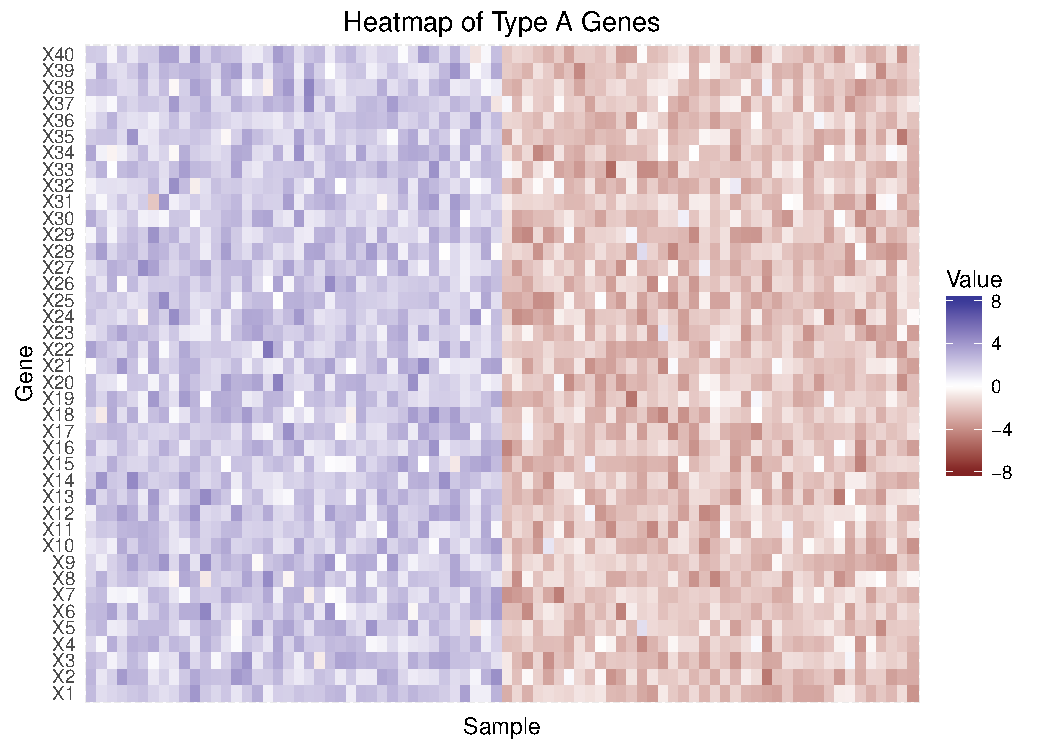
\includegraphics[width = \textwidth]{figures/Type_A_Gene.pdf}
    \caption{Type A: genes with class label but not with batch label signal.}
    \label{fig:type_a}
    \end{subfigure}
    ~
    \centering
    \begin{subfigure}[t]{0.4\textwidth}
    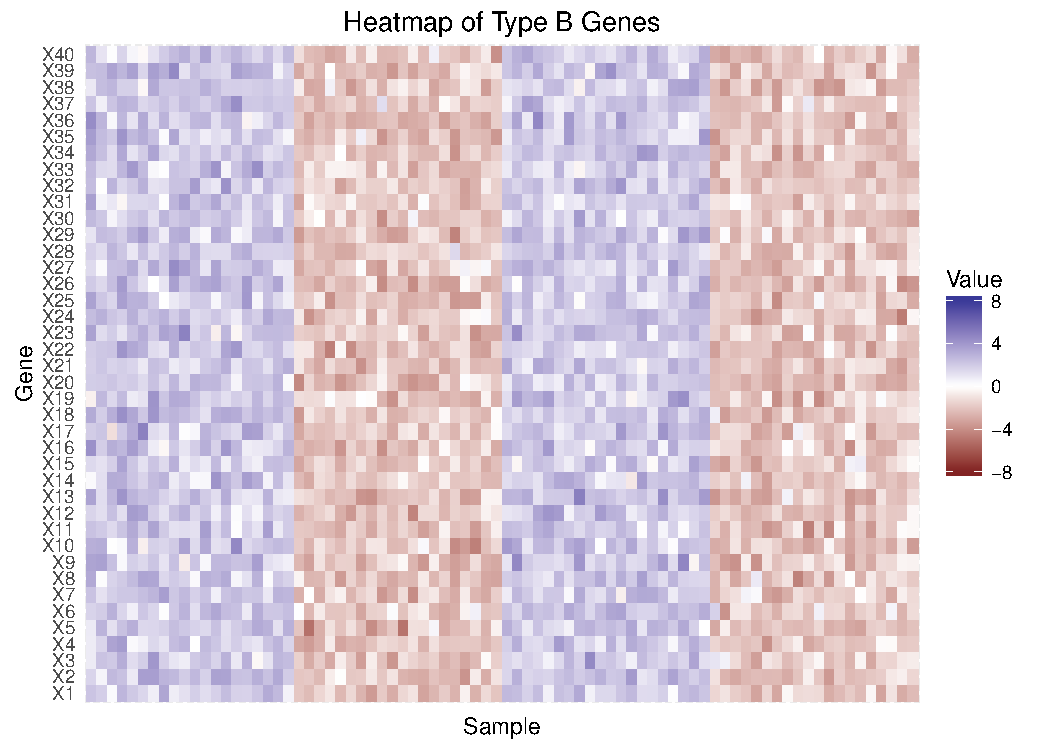
\includegraphics[width = \textwidth]{figures/Type_B_Gene.pdf}
    \caption{Type B: genes with batch label but not with class label signal.}
    \label{fig:type_b}
    \end{subfigure}
    \\
    \centering
    \begin{subfigure}[t]{0.4\textwidth}
    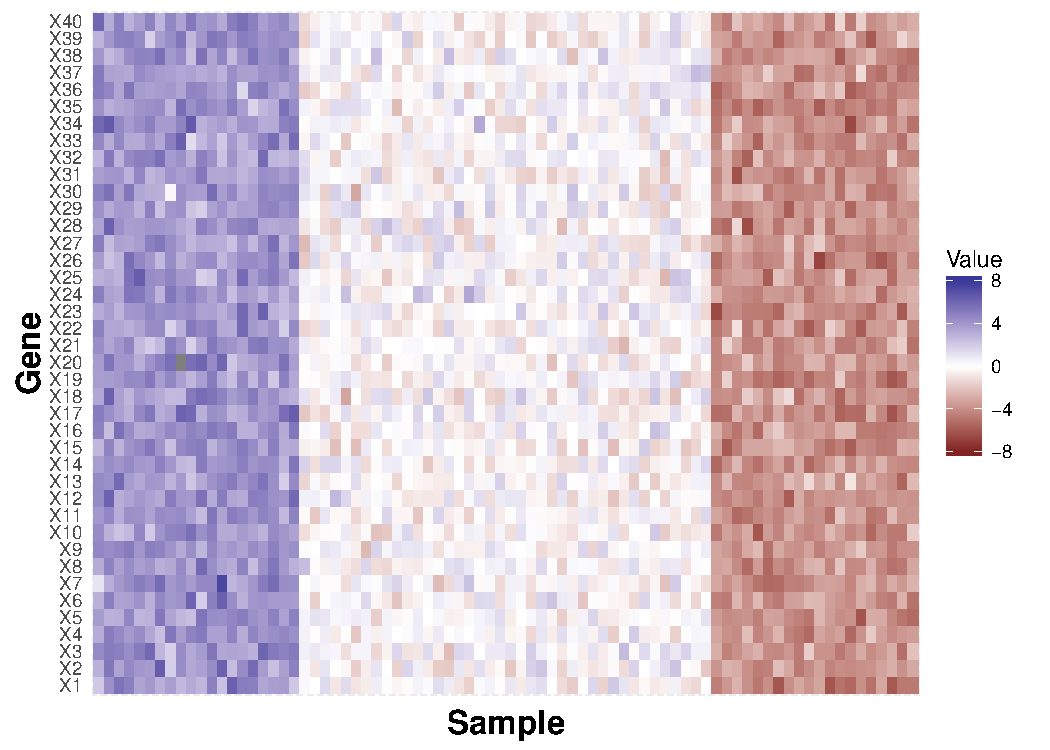
\includegraphics[width = \textwidth]{figures/Type_C_Gene.pdf}
    \caption{Type C: genes with both class and batch label signal.}
     \label{fig:type_c}
   \end{subfigure}
    ~
    \centering
    \begin{subfigure}[t]{0.4\textwidth}
    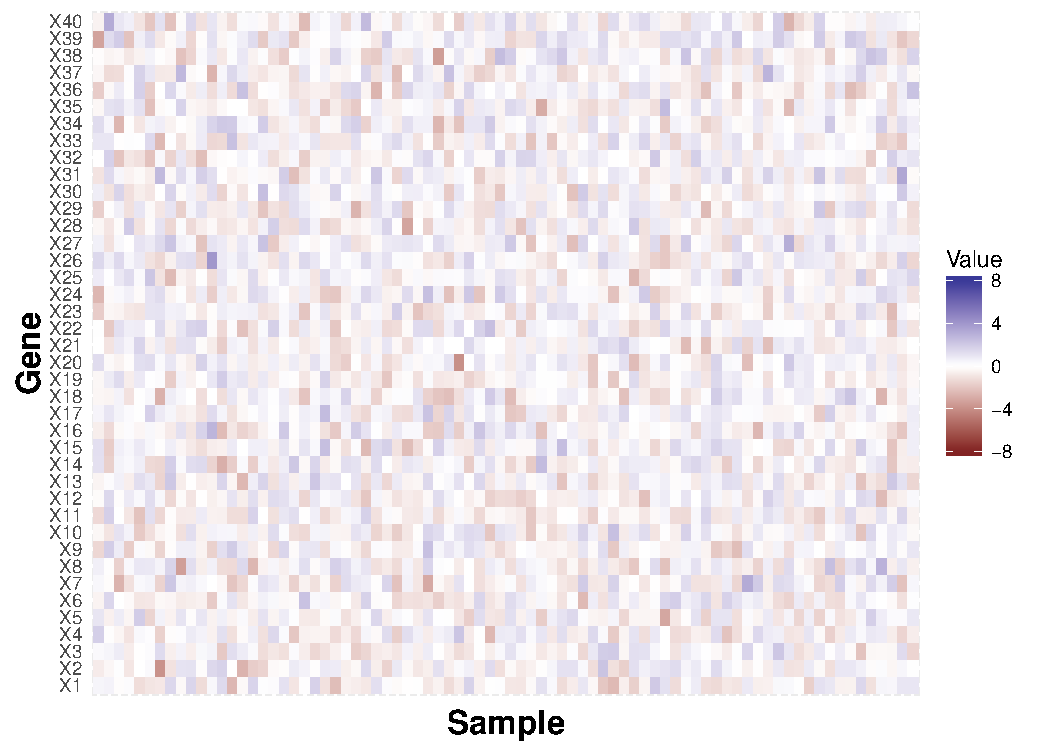
\includegraphics[width = \textwidth]{figures/Type_D_Gene.pdf}
    \caption{Type D: genes with no signal.}
    \label{fig:type_d}
    \end{subfigure}
    \caption{Separate heatmaps for each of the four gene types}
    \label{fig:heatmap}
\end{figure}



\newpage
\section{Simulation Result}

\subsection{Case 1: The simulation data set contains only Type C Genes and Type D Genes.}

The input data matrix in Case 1 is shown in Figure~\ref{fig:svas1}\subref{fig:data1}, which is the contamination of the matrices in Figure~\ref{fig:heatmap}\subref{fig:type_c} and Figure~\ref{fig:heatmap}\subref{fig:type_d}. Figure~\ref{fig:svas1}\subref{fig:sva1} shows that the data matrix after removing batch effects through IRW-SVA still remains the same pattern as the original simulation data set, which indicates that IRW-SVA fails to adjust batch effects in this case. Figure~\ref{fig:svas1}\subref{fig:new_sva1} shows that after removing the batch effects through modified SVA, the rows of Type C genes in the data set, which affected by both class and batch effects, have been recovered as the class signal in Figure~\ref{fig:heatmap}\subref{fig:type_a}. This from indicates that modified SVA adjusts batch effects and recovers the pattern of measured factor quite well in Case 1. 

In order to understand the failure of IRW-SVA in Case 1, the posterior probabilities are investigated in the two approaches to SVA. In Figure~\ref{fig:visual1}, the x-axis and y-axis represent gene index and probability respectively, and the genes are colored by their types. Figure~\ref{fig:visual1}\subref{fig:pprob1_1} and Figure~\ref{fig:visual1}\subref{fig:pprob1_2} show the posterior probability of each gene affected by class effects and batch effects respectively. Then in both sub-figures we expect that Type C genes have high probabilities while Type D genes have low probabilities. Figure~\ref{fig:visual1}\subref{fig:pprob1_1} indicates that both IRW-SVA and modified SVA correctly identify the genes affected by class effects. The left panel of Figure~\ref{fig:visual1}\subref{fig:pprob1_2} shows that IRW-SVA can not correctly identify the genes associated with batch label, while the right panel of Figure~\ref{fig:visual1}\subref{fig:pprob1_2} indicates modified SVA is able to do that. This is not surprised since IRW-SVA relies on Type B Genes to recover the signal of batch effects but the data set in Case 1 does not contain Type B genes.

Moreover, Figure~\ref{fig:vector1} visualizes the scores of samples on the surrogate variable constructed by the two approaches to SVA respectively. In Figure~\ref{fig:vector1}, x-axis and y-axis represent samples and expression value respectively, and samples are colored by batch labels. The right panel of Figure~\ref{fig:vector1} shows samples from two batches are more separable under the direction of surrogate variable gained from modified SVA. 

All these results in the Case 1 indicate that modified SVA has better performance than IRW-SVA when Type B genes do not exist in the data.

\begin{figure}[h!]
    \centering
    \begin{subfigure}[b]{0.31\textwidth}
        \centering
        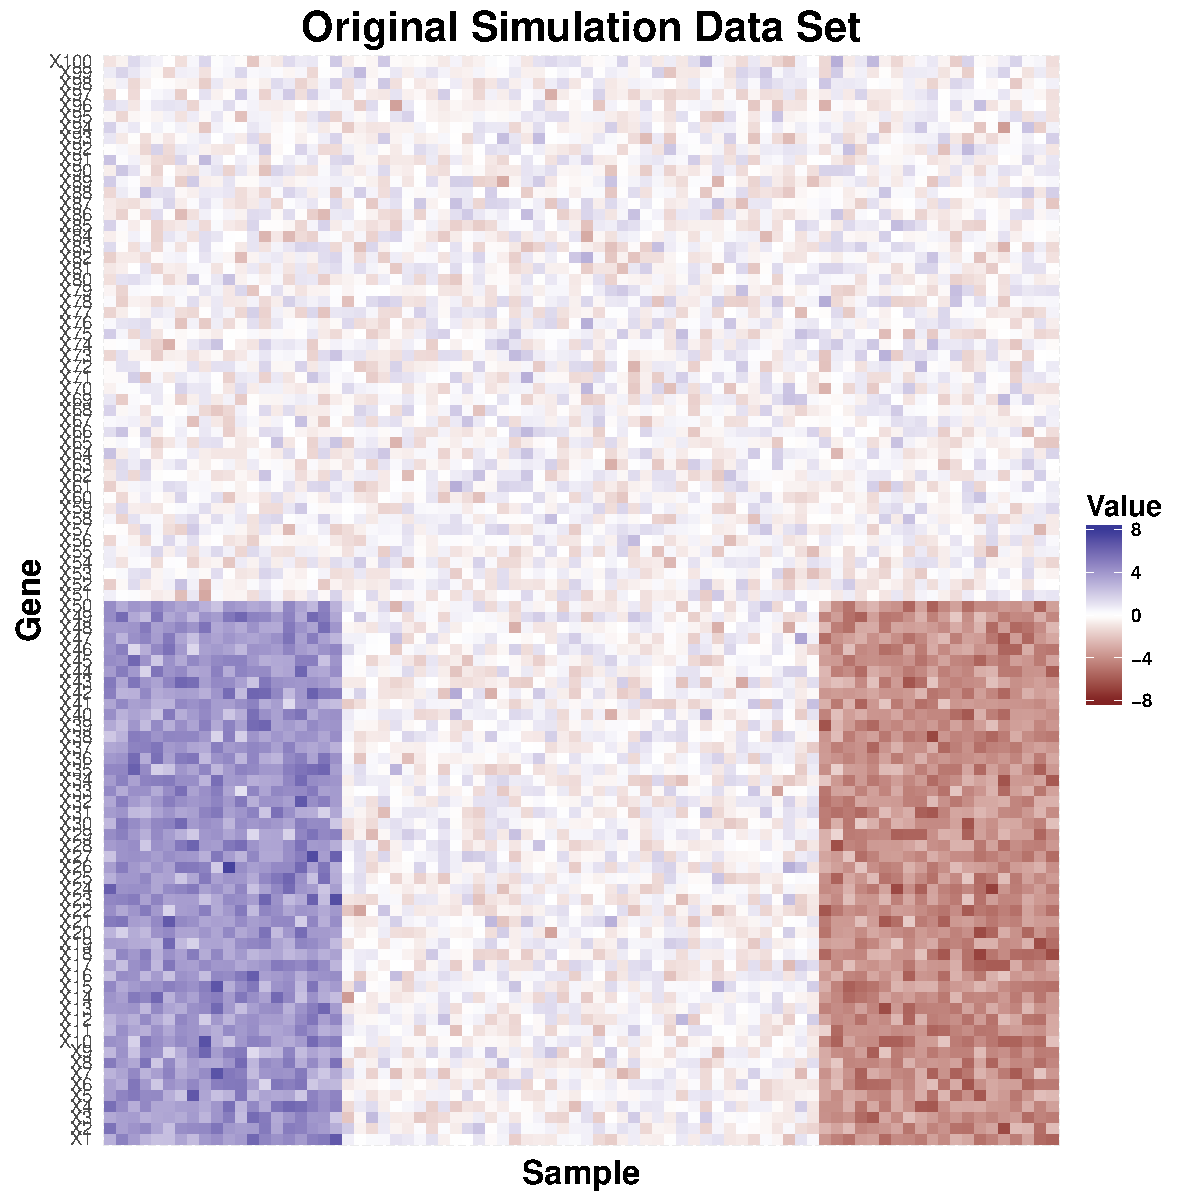
\includegraphics[width = \textwidth]{figures/simulate1.pdf}
        \caption{Original simulation data set in the Case 1}
        \label{fig:data1}
    \end{subfigure}% 
~
    \begin{subfigure}[b]{0.31\textwidth}
        \centering
        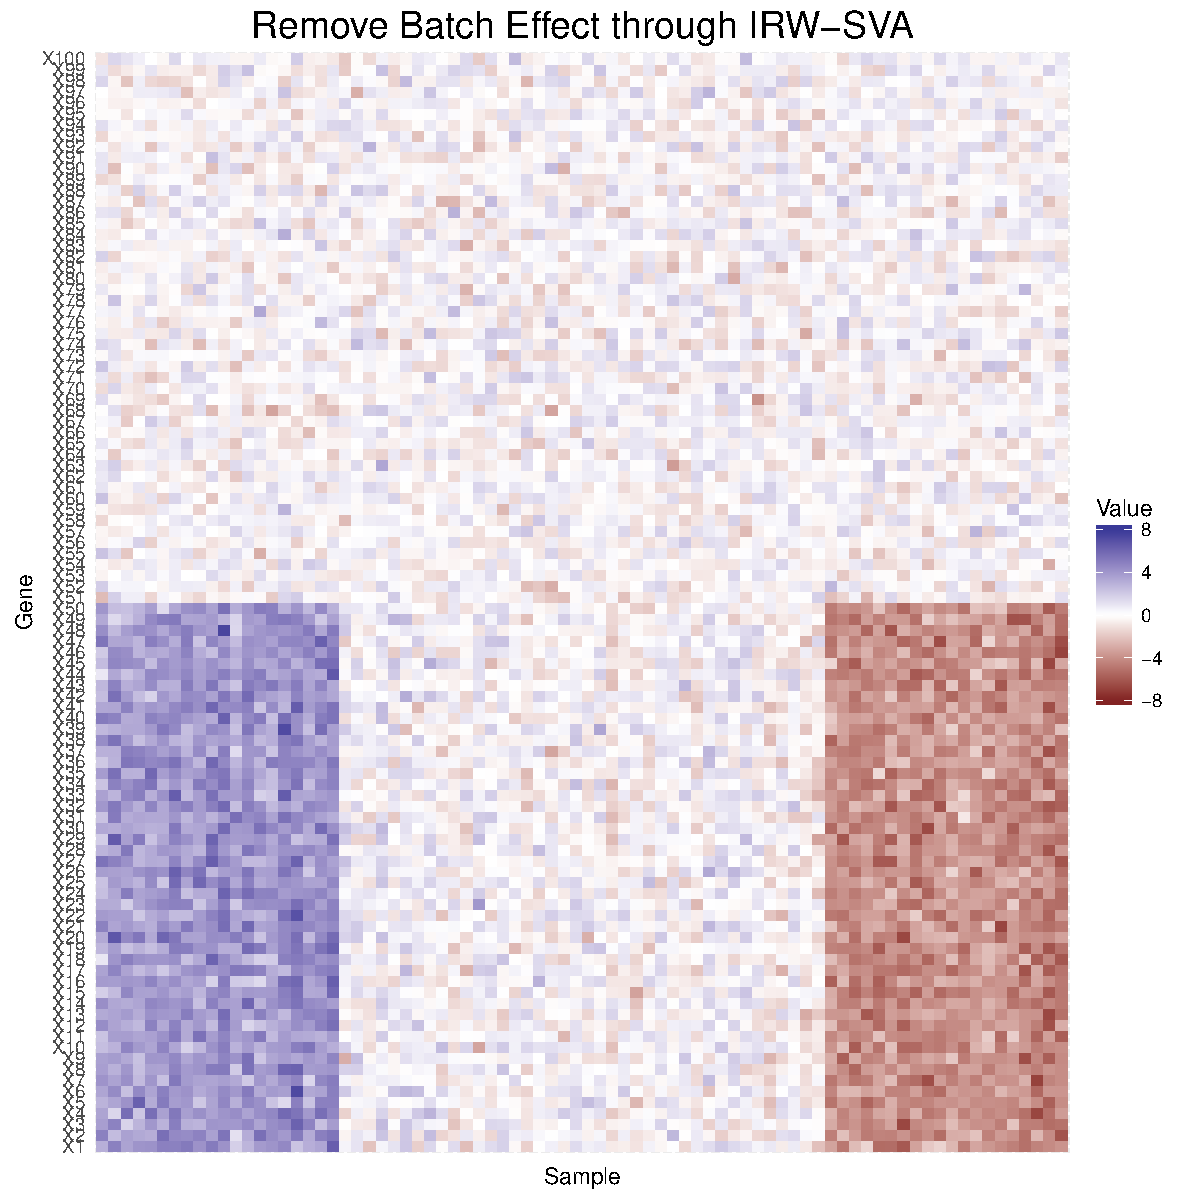
\includegraphics[width = \textwidth]{figures/sva1.pdf}
        \caption{Remove batch effect through IRW-SVA}
        \label{fig:sva1}
    \end{subfigure}  %
~
    \begin{subfigure}[b]{0.31\textwidth}
        \centering
        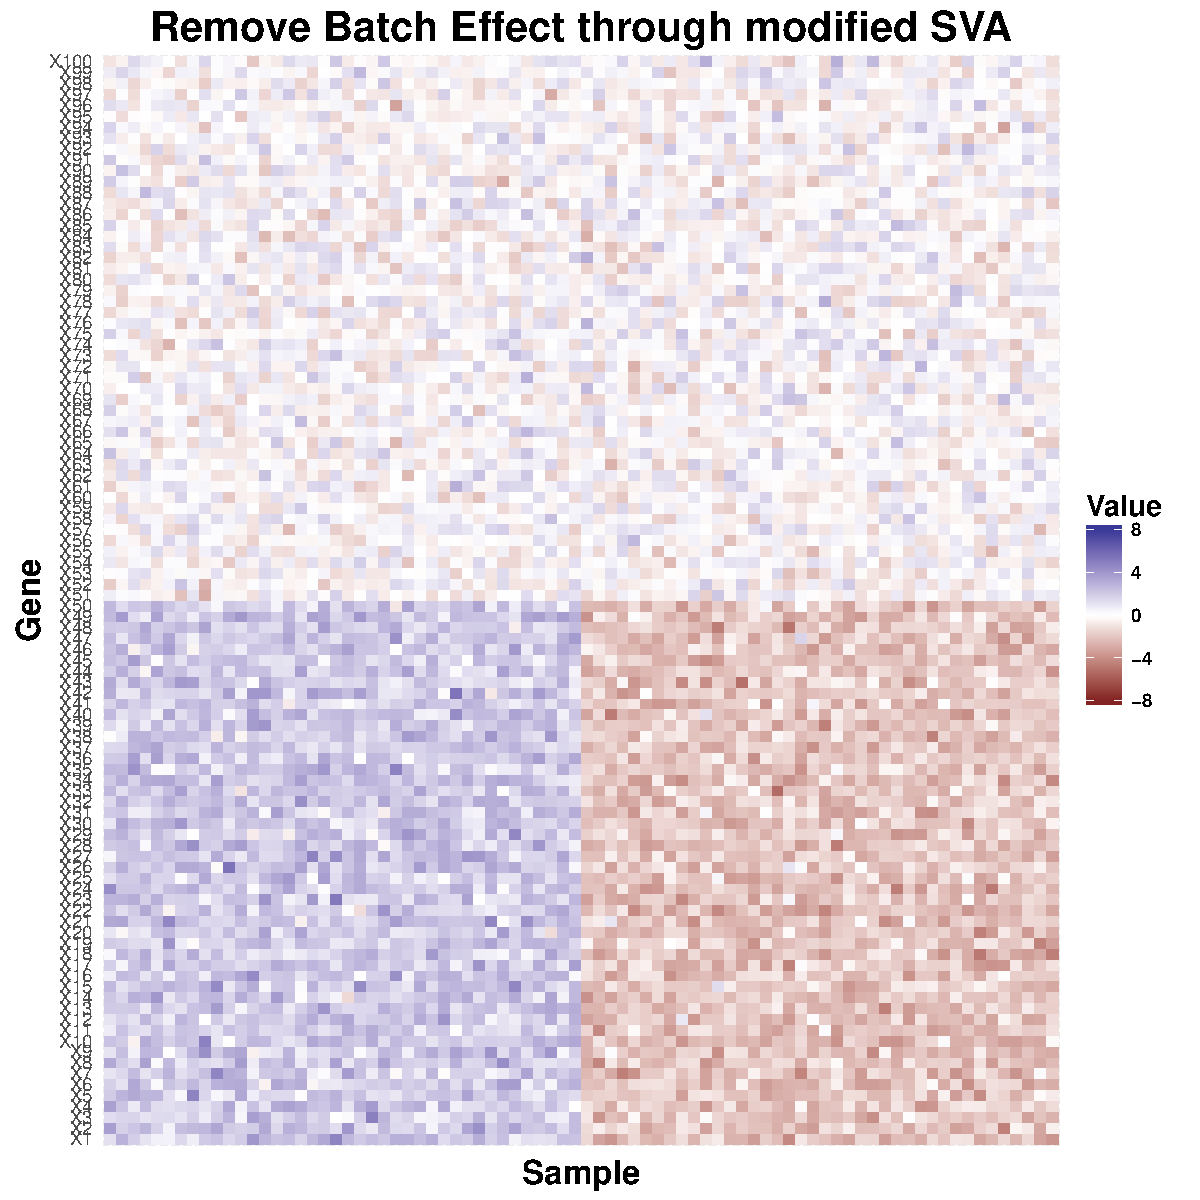
\includegraphics[width = \textwidth]{figures/new_sva1.pdf}
        \caption{Remove batch effect through modified SVA}
        \label{fig:new_sva1}
    \end{subfigure}    
    \caption{Study batch effect through two approaches to SVA in Case 1}
    \label{fig:svas1}
\end{figure}




\begin{figure}[h!]
    \centering
    \begin{subfigure}[t]{0.45\textwidth}
    \centering
    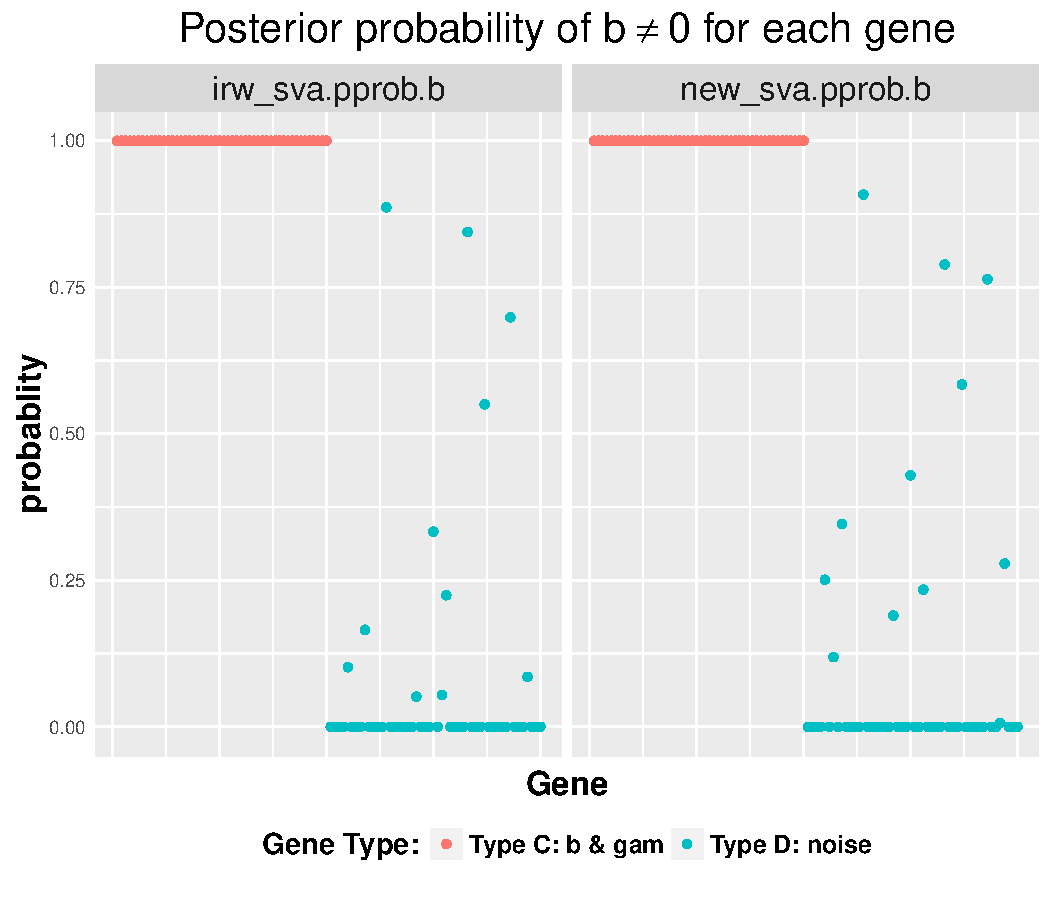
\includegraphics[width = \textwidth]{figures/pprop1_2.pdf}
    \caption{Posterior probability of genes affected by class label (measured factor).}
    \label{fig:pprob1_1}
    \end{subfigure}
    ~
     \begin{subfigure}[t]{0.45\textwidth}
    \centering
    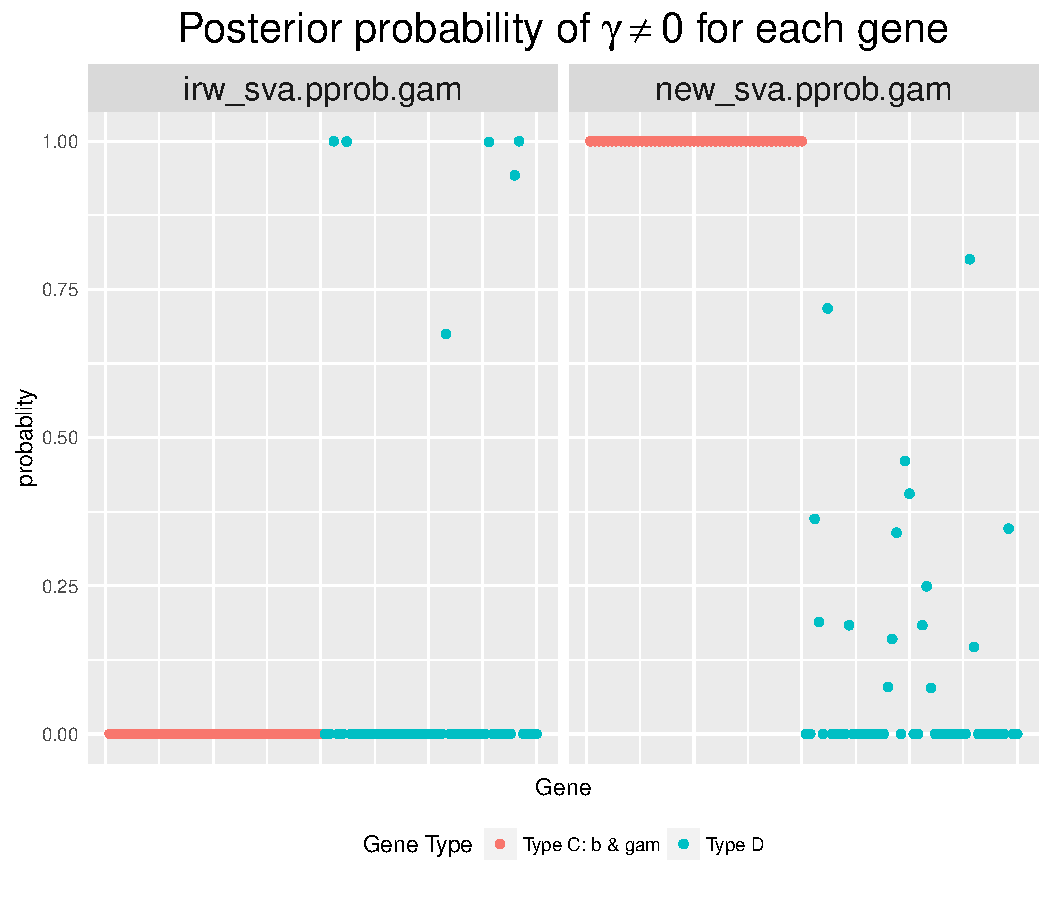
\includegraphics[width = \textwidth]{figures/pprop1_1.pdf}
    \caption{Posterior probability of genes affected by batch label (unmeasured factor).}
    \label{fig:pprob1_2}
    \end{subfigure}
    \caption{Visualize the posterior probabilities for genes in the Case 1. In each subfigure, the panels on the left show the results from IRW-SVA and the panels on the right show the results form modified SVA.}
    \label{fig:visual1}
\end{figure}

\begin{figure}
    \centering
    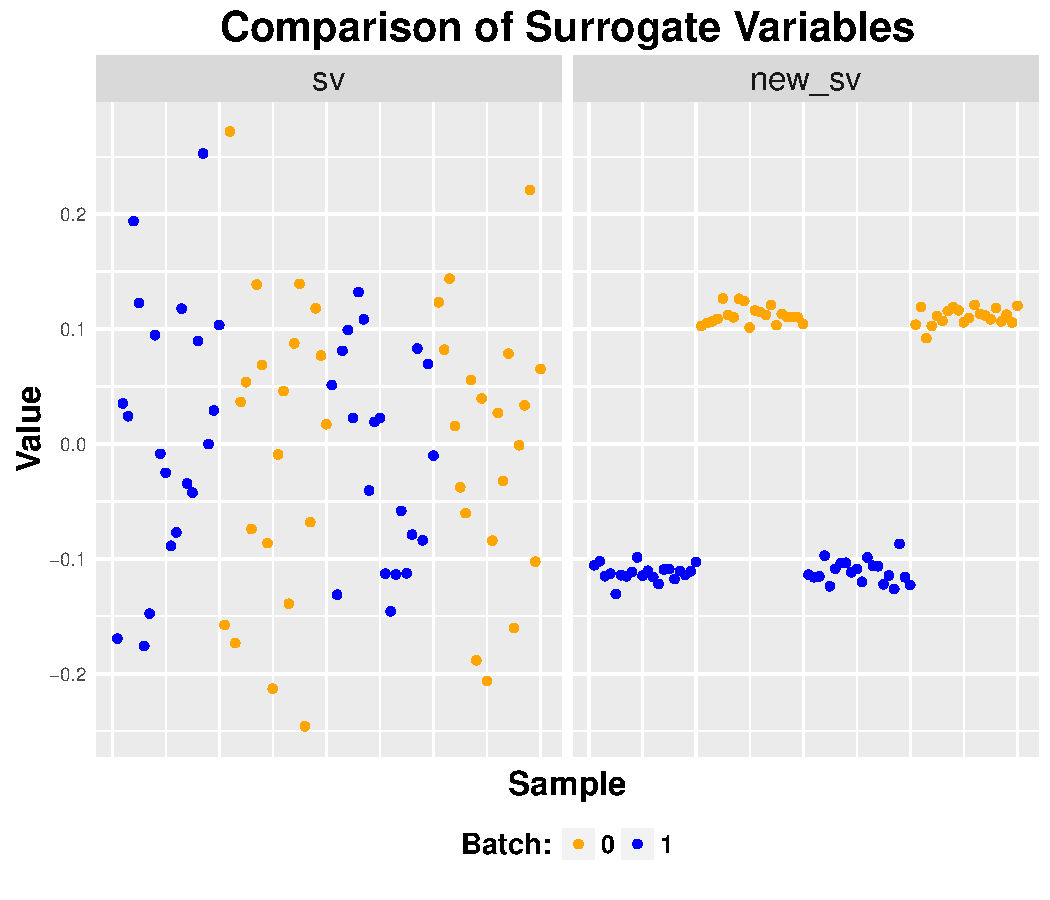
\includegraphics[width = 0.6\textwidth]{figures/vector1.pdf}
    \caption{Comparison of surrogate variables. The left panel shows the surrogate variable constructed through IRW-SVA and the right panel shows the surrogate variable constructed through modified SVA.}
    \label{fig:vector1}
\end{figure}

\newpage

\subsection{Case 2: The simulation data set contains all four types of genes.}

In contrast to Case 1, the input data matrix in Case 2 contains all four types of genes, as shown in Figure~\ref{fig:svas2}\subref{fig:data2}, which is a typical situation we expect IRW-SVA works. Figure~\ref{fig:svas2}\subref{fig:sva2} and Figure~\ref{fig:svas2}\subref{fig:new_sva2} shows that the genes affected by class labels in the two adjusted data matrices have the same pattern in Figure~\ref{fig:heatmap}\subref{fig:type_a}. There results demonstrate that both IRW-SVA and modified SVA can adjust the batch effects in Case 2.  

Moreover, Figure~\ref{fig:visual2} shows the posterior probabilities in the two approaches. In Case 2, we expect that Type A and Type C genes have high posterior probabilities affected by class effects in Figure~\ref{fig:visual2}\subref{fig:pprob2_1}, and Type B and Type C genes  have high posterior probabilities affected by batch effects in Figure~\ref{fig:visual2}\subref{fig:pprob2_2}. Then Figure~\ref{fig:visual2}\subref{fig:pprob2_1} and Figure~\ref{fig:visual2}\subref{fig:pprob2_2} shows that both IRW-SVA and modified SVA are able to identify the genes associated with batch label and class label as well. 

The scores of samples on the surrogate variables from two approaches to SVA are shown in Figure~\ref{fig:vector2}. As shown in Figure~\ref{fig:vector2}, two approaches to SVA produce similar surrogate variables which separate samples from two batches pretty well.

To sum up, the simulation results in the Case 2 indicate that IRW-SVA and modified SVA have similar performance and are able to adjust the unmeasured factors when the data set contains Type B genes.

\begin{figure}[h!]
    \centering
    \begin{subfigure}[b]{0.31\textwidth}
        \centering
        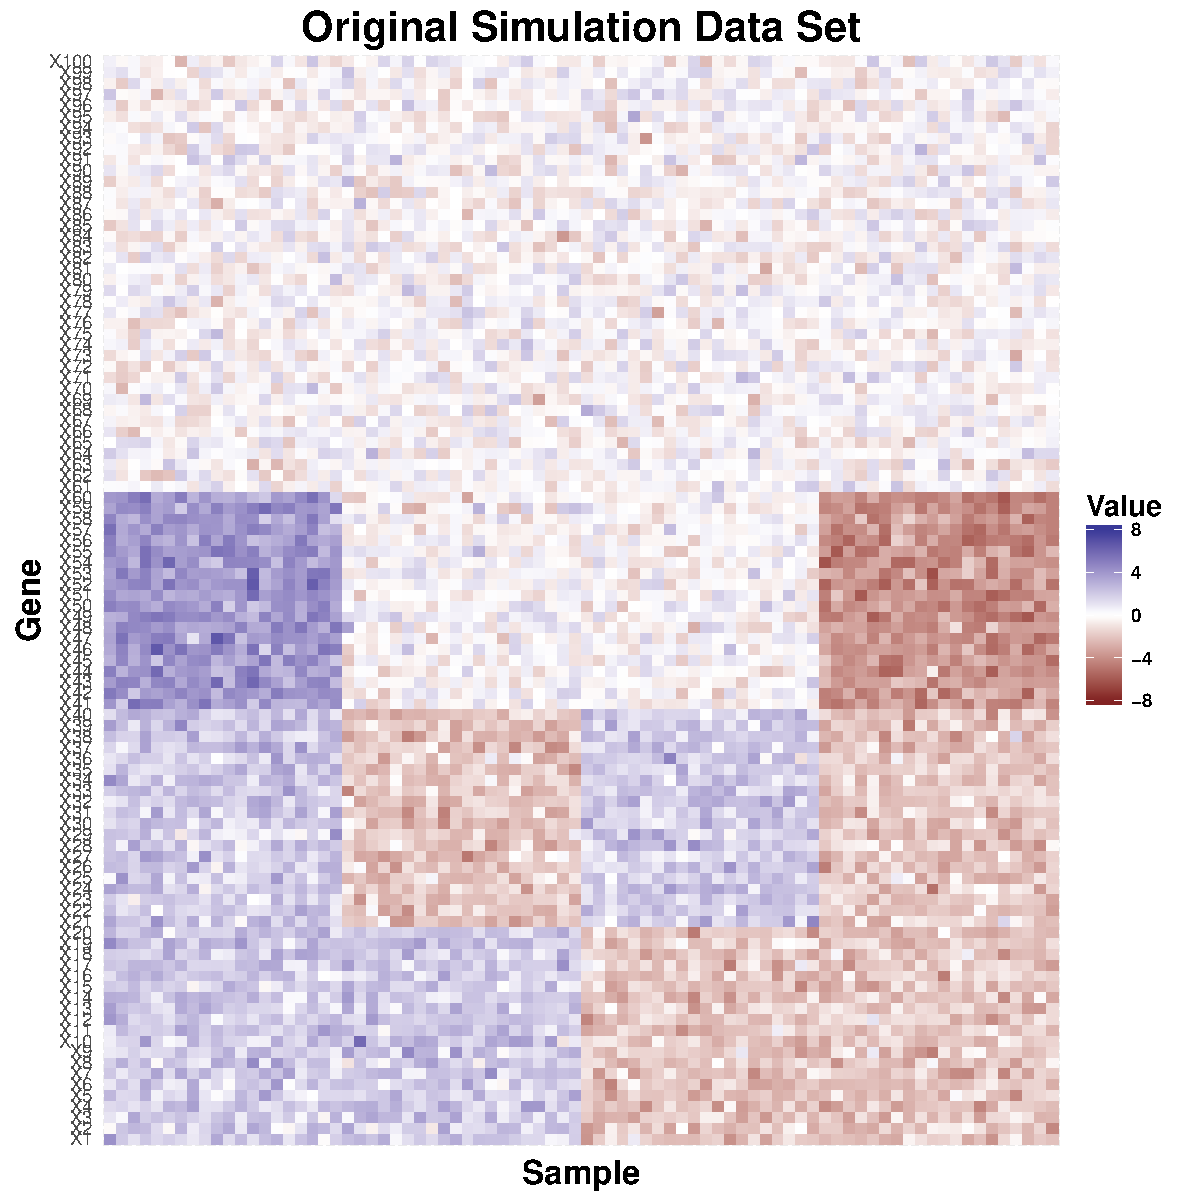
\includegraphics[width = \textwidth]{figures/simulate2.pdf}
        \caption{Original simulation data set in the Case 2}
        \label{fig:data2}
    \end{subfigure}% 
~
    \begin{subfigure}[b]{0.31\textwidth}
        \centering
        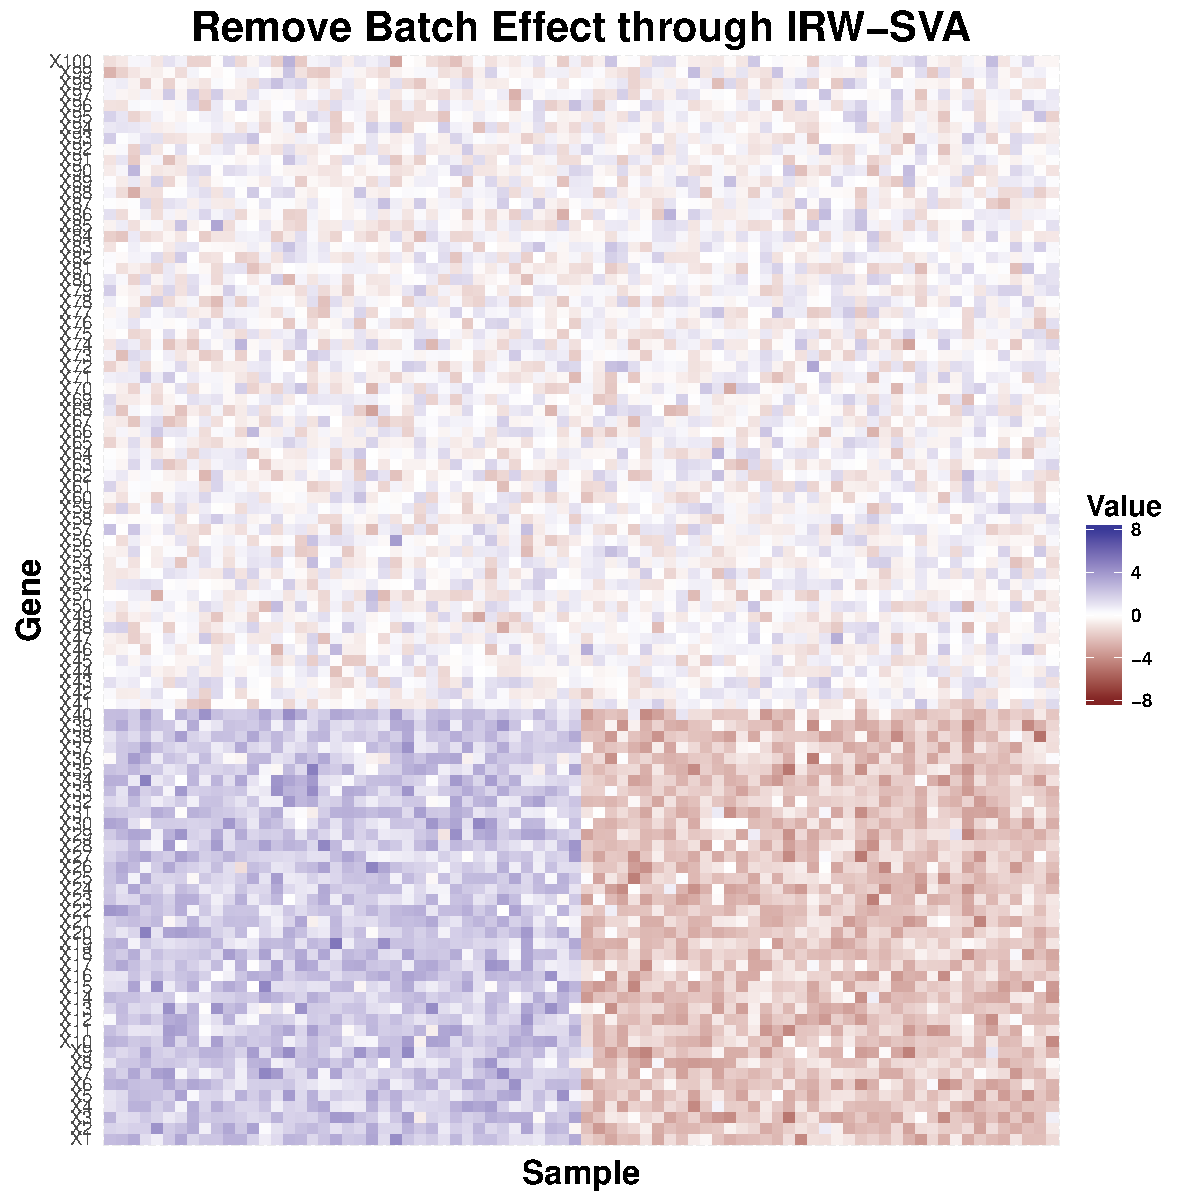
\includegraphics[width = \textwidth]{figures/sva2.pdf}
        \caption{Remove batch effect through IRW-SVA}
        \label{fig:sva2}
    \end{subfigure}  %
~
    \begin{subfigure}[b]{0.31\textwidth}
        \centering
        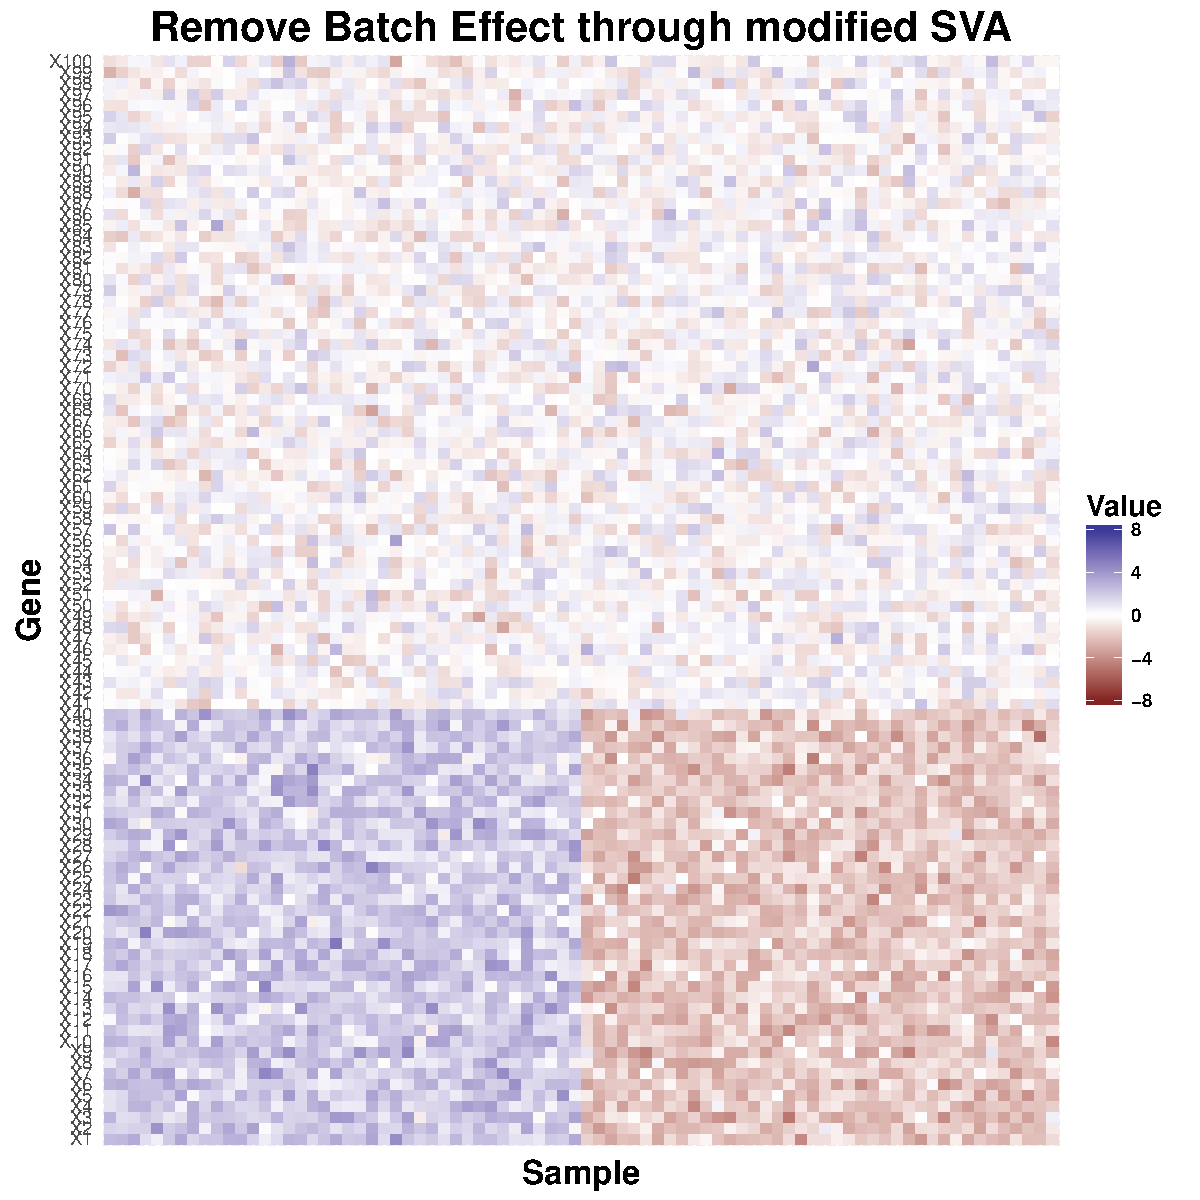
\includegraphics[width = \textwidth]{figures/new_sva2.pdf}
        \caption{Remove batch effect through modified SVA}
        \label{fig:new_sva2}
    \end{subfigure}    
    \caption{Study batch effect through two approaches to SVA in Case 2}
    \label{fig:svas2}
\end{figure}




\begin{figure}[h!]
    \centering
    \begin{subfigure}[t]{0.45\textwidth}
    \centering
    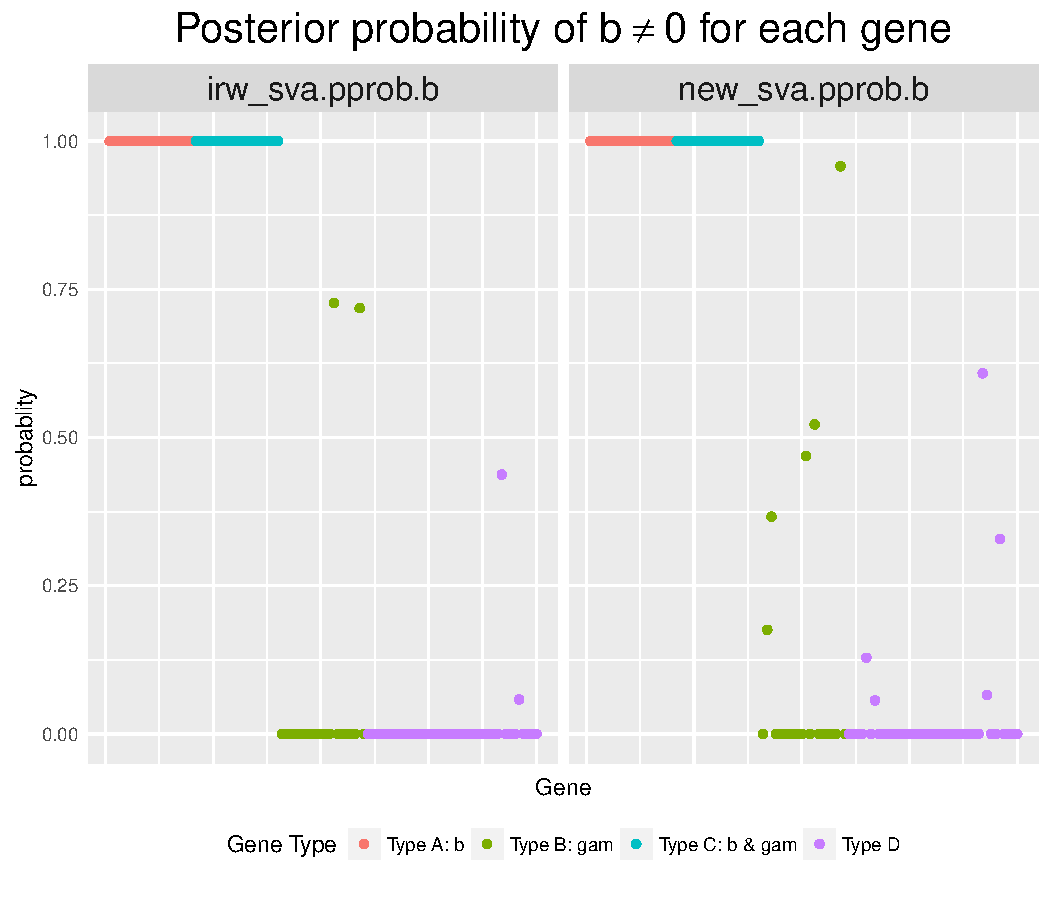
\includegraphics[width = \textwidth]{figures/pprop2_2.pdf}
    \caption{Posterior probability of genes affected by class label (measured factor).}
    \label{fig:pprob2_1}
    \end{subfigure}
    ~
     \begin{subfigure}[t]{0.45\textwidth}
    \centering
    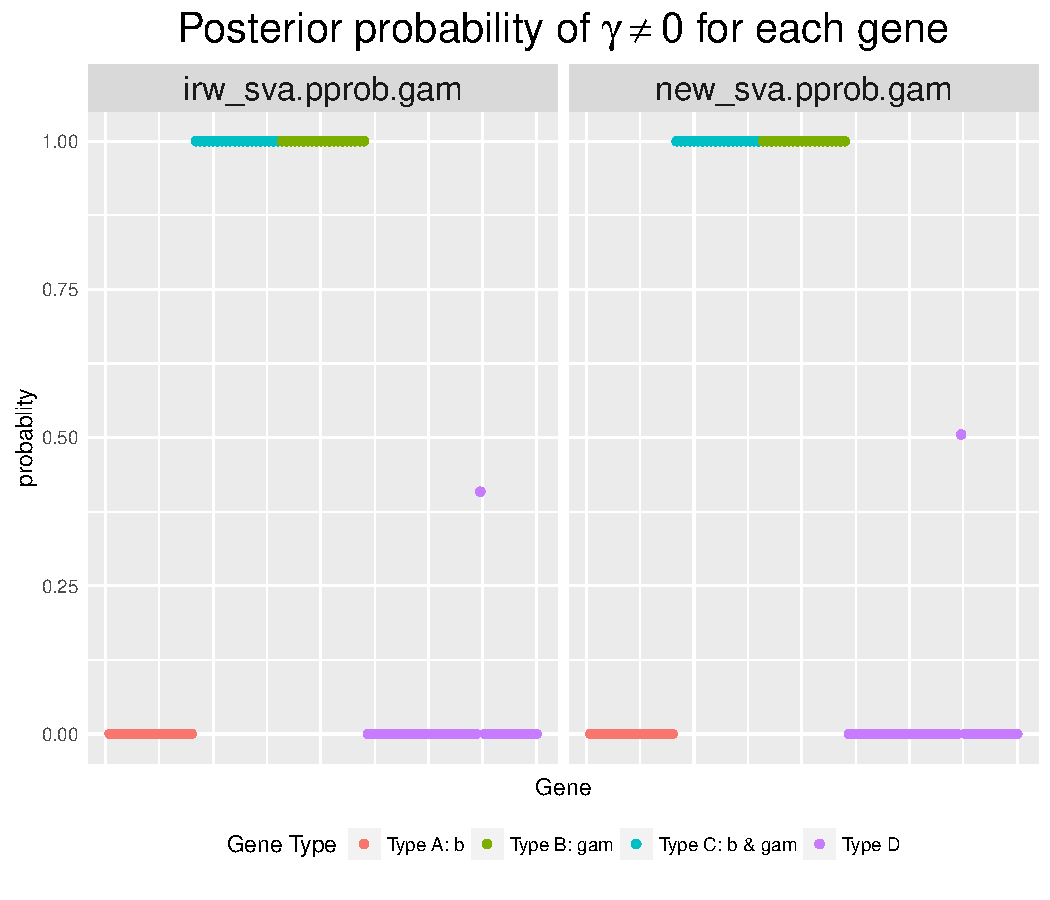
\includegraphics[width = \textwidth]{figures/pprop2_1.pdf}
    \caption{Posterior probability of genes affected by batch label (unmeasured factor).}
    \label{fig:pprob2_2}
    \end{subfigure}
    \caption{Visualize the posterior probabilities for genes in the Case 2. In each subfigure, the panels on the left show the results from IRW-SVA and the panels on the right show the results form modified SVA.}
    \label{fig:visual2}
\end{figure}

\begin{figure}
    \centering
    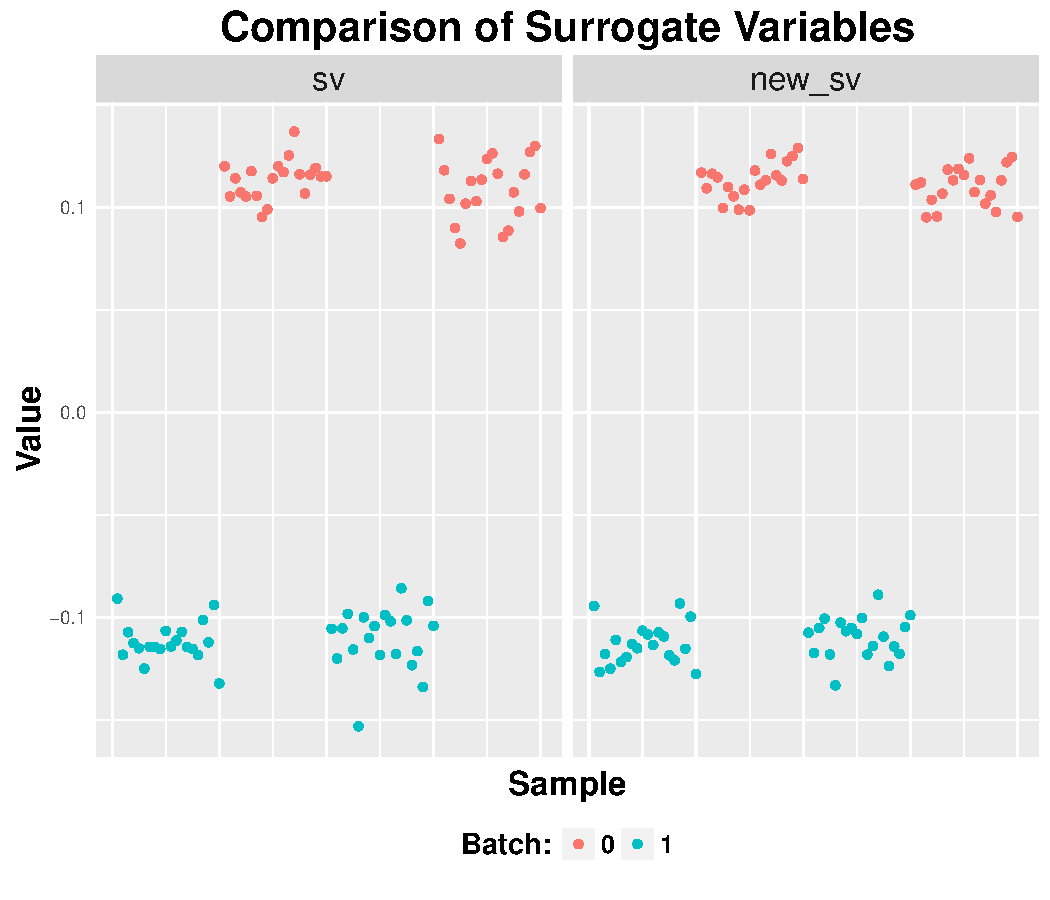
\includegraphics[width = 0.6\textwidth]{figures/vector2.pdf}
    \caption{Comparison of surrogate variables. The left panel shows the surrogate variable constructed through IRW-SVA and the right panel shows the surrogate variable constructed through modified SVA.}
    \label{fig:vector2}
\end{figure}

\newpage
\clearpage

\bibliographystyle{plain}
\bibliography{svabib}

\end{document}